%% fig_efourshifts.tex   (generated by make_round40.py; do not edit by hand)
%% Shifts along chains at n = 4 and the two-shift theorem (lem:efourshifts, thm:efourtwolevels).
\documentclass[tikz,border=8pt]{standalone}
\usepackage{amsmath,amssymb}
\usetikzlibrary{arrows.meta,calc,decorations.pathreplacing}
%% palette.tex -- shared colour definitions for the figures
\definecolor{PInk}{RGB}{26,32,44}
\definecolor{PBlue}{RGB}{37,82,139}
\definecolor{PTeal}{RGB}{23,127,125}
\definecolor{POchre}{RGB}{193,138,44}
\definecolor{PClay}{RGB}{178,74,58}
\definecolor{PSlate}{RGB}{108,122,137}
\definecolor{PViolet}{RGB}{110,86,150}
\definecolor{WBlue}{RGB}{223,234,246}
\definecolor{WTeal}{RGB}{220,238,236}
\definecolor{WOchre}{RGB}{250,240,218}
\definecolor{WClay}{RGB}{247,229,224}
\definecolor{WSlate}{RGB}{238,241,244}
\definecolor{PMag}{RGB}{158,58,110}
\definecolor{PGrass}{RGB}{62,124,66}
\definecolor{PAmber}{RGB}{214,112,38}
\definecolor{PIndigo}{RGB}{58,64,140}
\definecolor{PRule}{RGB}{176,186,197}

%% shared macros so the standalone figures match the paper
\providecommand{\QQ}{\mathbb{Q}}
\providecommand{\ZZ}{\mathbb{Z}}
\providecommand{\RR}{\mathbb{R}}
\providecommand{\CC}{\mathbb{C}}
\providecommand{\PP}{\mathbb{P}}
\providecommand{\Kx}{K^{\times}}
\providecommand{\HW}{W}
\providecommand{\Nm}{\mathrm{N}}
\providecommand{\Hdg}{\mathrm{Hdg}}
\providecommand{\NS}{\mathrm{NS}}
\providecommand{\cA}{\mathcal{A}}
\providecommand{\cD}{\mathcal{D}}
\providecommand{\cF}{\mathcal{F}}
\providecommand{\cP}{\mathcal{P}}
\providecommand{\cO}{\mathcal{O}}
\providecommand{\cQ}{\mathcal{Q}}
\providecommand{\bbar}[1]{\overline{#1}}
\providecommand{\ch}{\operatorname{ch}}
\providecommand{\End}{\mathrm{End}}
\providecommand{\Ext}{\operatorname{Ext}}
\providecommand{\Supp}{\operatorname{Supp}}

\begin{document}
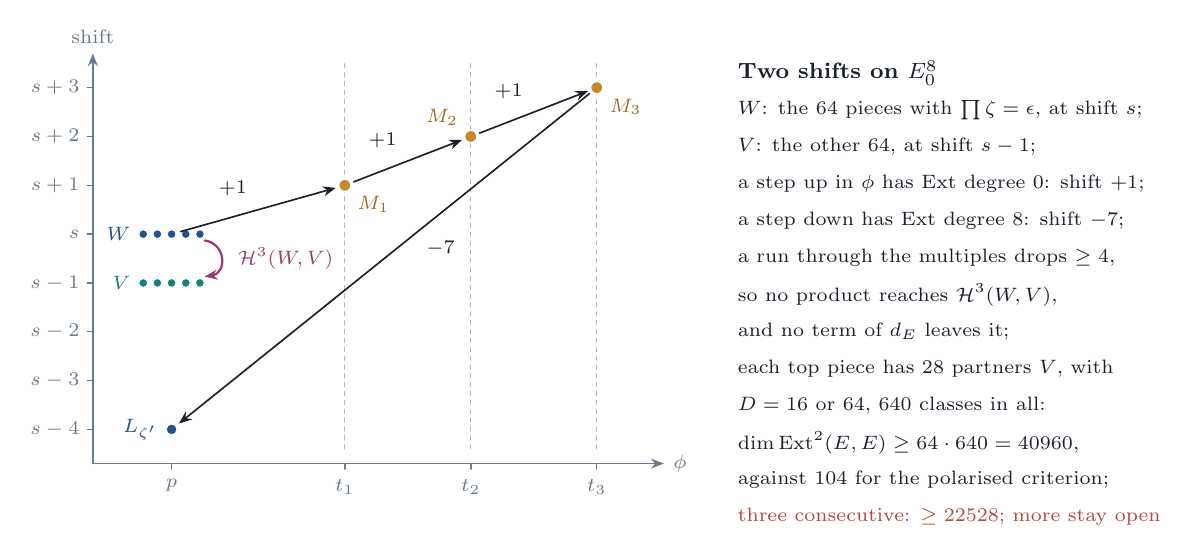
\begin{tikzpicture}[x=1cm,y=1cm,line join=round,line cap=round,
  font=\small,text=PInk,lbl/.style={inner sep=1pt}]
  \draw[PSlate,line width=0.5pt,-{Stealth[length=4.6pt,width=3.6pt]}] (0.9500,0.0360) -- (0.9500,5.2440);
  \draw[PSlate,line width=0.5pt,-{Stealth[length=4.6pt,width=3.6pt]}] (0.9500,0.0360) -- (8.2000,0.0360);
  \draw[PSlate,line width=0.5pt] (0.8800,0.4700) -- (0.9500,0.4700);
  \draw[PSlate,line width=0.5pt] (0.8800,1.0900) -- (0.9500,1.0900);
  \draw[PSlate,line width=0.5pt] (0.8800,1.7100) -- (0.9500,1.7100);
  \draw[PSlate,line width=0.5pt] (0.8800,2.3300) -- (0.9500,2.3300);
  \draw[PSlate,line width=0.5pt] (0.8800,2.9500) -- (0.9500,2.9500);
  \draw[PSlate,line width=0.5pt] (0.8800,3.5700) -- (0.9500,3.5700);
  \draw[PSlate,line width=0.5pt] (0.8800,4.1900) -- (0.9500,4.1900);
  \draw[PSlate,line width=0.5pt] (0.8800,4.8100) -- (0.9500,4.8100);
  \draw[PSlate,line width=0.5pt] (1.9500,0.0360) -- (1.9500,-0.0340);
  \draw[PSlate,line width=0.5pt] (4.1500,0.0360) -- (4.1500,-0.0340);
  \draw[PSlate,line width=0.5pt] (5.7500,0.0360) -- (5.7500,-0.0340);
  \draw[PSlate,line width=0.5pt] (7.3500,0.0360) -- (7.3500,-0.0340);
  \draw[PRule,line width=0.35pt,dash pattern=on 1.6pt off 1.6pt] (4.1500,0.2220) -- (4.1500,5.1200);
  \draw[PRule,line width=0.35pt,dash pattern=on 1.6pt off 1.6pt] (5.7500,0.2220) -- (5.7500,5.1200);
  \draw[PRule,line width=0.35pt,dash pattern=on 1.6pt off 1.6pt] (7.3500,0.2220) -- (7.3500,5.1200);
  \path[fill=PBlue,draw=white,line width=0.35pt] (1.5900,2.9500) circle (1.60pt);
  \path[fill=PBlue,draw=white,line width=0.35pt] (1.7700,2.9500) circle (1.60pt);
  \path[fill=PBlue,draw=white,line width=0.35pt] (1.9500,2.9500) circle (1.60pt);
  \path[fill=PBlue,draw=white,line width=0.35pt] (2.1300,2.9500) circle (1.60pt);
  \path[fill=PBlue,draw=white,line width=0.35pt] (2.3100,2.9500) circle (1.60pt);
  \path[fill=PTeal,draw=white,line width=0.35pt] (1.5900,2.3300) circle (1.60pt);
  \path[fill=PTeal,draw=white,line width=0.35pt] (1.7700,2.3300) circle (1.60pt);
  \path[fill=PTeal,draw=white,line width=0.35pt] (1.9500,2.3300) circle (1.60pt);
  \path[fill=PTeal,draw=white,line width=0.35pt] (2.1300,2.3300) circle (1.60pt);
  \path[fill=PTeal,draw=white,line width=0.35pt] (2.3100,2.3300) circle (1.60pt);
  \draw[PMag,line width=0.8pt,-{Stealth[length=4.6pt,width=3.6pt]}] (2.3700,2.8700) .. controls (2.6500,2.8260) and (2.6500,2.4540) .. (2.3700,2.4100);
  \draw[PInk,line width=0.6pt,-{Stealth[length=4.6pt,width=3.6pt]}] (2.0655,2.9826) -- (4.0345,3.5374);
  \draw[PInk,line width=0.6pt,-{Stealth[length=4.6pt,width=3.6pt]}] (4.2619,3.6134) -- (5.6381,4.1466);
  \draw[PInk,line width=0.6pt,-{Stealth[length=4.6pt,width=3.6pt]}] (5.8619,4.2334) -- (7.2381,4.7666);
  \draw[PInk,line width=0.6pt,-{Stealth[length=4.6pt,width=3.6pt]}] (7.2565,4.7348) -- (2.0435,0.5452);
  \path[fill=POchre,draw=white,line width=0.45pt] (4.1500,3.5700) circle (2.20pt);
  \path[fill=POchre,draw=white,line width=0.45pt] (5.7500,4.1900) circle (2.20pt);
  \path[fill=POchre,draw=white,line width=0.45pt] (7.3500,4.8100) circle (2.20pt);
  \path[fill=PBlue,draw=white,line width=0.45pt] (1.9500,0.4700) circle (2.00pt);
  \node[lbl,anchor=south,text=PSlate,font=\scriptsize] at (0.9500,5.3240) {shift};
  \node[lbl,anchor=west,text=PSlate,font=\scriptsize] at (8.2800,0.0360) {$\phi$};
  \node[lbl,anchor=east,text=PSlate,font=\scriptsize] at (0.8200,0.4700) {$s-4$};
  \node[lbl,anchor=east,text=PSlate,font=\scriptsize] at (0.8200,1.0900) {$s-3$};
  \node[lbl,anchor=east,text=PSlate,font=\scriptsize] at (0.8200,1.7100) {$s-2$};
  \node[lbl,anchor=east,text=PSlate,font=\scriptsize] at (0.8200,2.3300) {$s-1$};
  \node[lbl,anchor=east,text=PSlate,font=\scriptsize] at (0.8200,2.9500) {$s$};
  \node[lbl,anchor=east,text=PSlate,font=\scriptsize] at (0.8200,3.5700) {$s+1$};
  \node[lbl,anchor=east,text=PSlate,font=\scriptsize] at (0.8200,4.1900) {$s+2$};
  \node[lbl,anchor=east,text=PSlate,font=\scriptsize] at (0.8200,4.8100) {$s+3$};
  \node[lbl,anchor=north,text=PSlate,font=\scriptsize] at (1.9500,-0.1240) {$p$};
  \node[lbl,anchor=north,text=PSlate,font=\scriptsize] at (4.1500,-0.1240) {$t_{1}$};
  \node[lbl,anchor=north,text=PSlate,font=\scriptsize] at (5.7500,-0.1240) {$t_{2}$};
  \node[lbl,anchor=north,text=PSlate,font=\scriptsize] at (7.3500,-0.1240) {$t_{3}$};
  \node[lbl,anchor=east,text=PBlue,font=\scriptsize] at (1.4700,2.9500) {$W$};
  \node[lbl,anchor=east,text=PTeal,font=\scriptsize] at (1.4700,2.3300) {$V$};
  \node[lbl,anchor=west,text=PMag,font=\scriptsize] at (2.7500,2.6400) {$\mathcal{H}^{3}(W,V)$};
  \node[lbl,anchor=west,text=POchre!80!black,font=\scriptsize] at (4.2700,3.3262) {$M_{1}$};
  \node[lbl,anchor=east,text=POchre!80!black,font=\scriptsize] at (5.6300,4.4338) {$M_{2}$};
  \node[lbl,anchor=west,text=POchre!80!black,font=\scriptsize] at (7.4700,4.5662) {$M_{3}$};
  \node[lbl,anchor=east,text=PBlue,font=\scriptsize] at (1.8100,0.4700) {$L_{\zeta'}$};
  \node[lbl,anchor=east,text=PInk,font=\scriptsize] at (2.9500,3.5261) {$+1$};
  \node[lbl,anchor=east,text=PInk,font=\scriptsize] at (4.8500,4.1461) {$+1$};
  \node[lbl,anchor=east,text=PInk,font=\scriptsize] at (6.4500,4.7661) {$+1$};
  \node[lbl,anchor=west,text=PInk,font=\scriptsize] at (5.1420,2.7711) {$-7$};
  \node[lbl,anchor=west,text=PInk,font=\footnotesize] at (9.1000,4.9960) {\textbf{Two shifts on $E_{0}^{8}$}};
  \node[lbl,anchor=west,text=PInk,font=\scriptsize] at (9.1000,4.5260) {$W$: the $64$ pieces with $\prod\zeta=\epsilon$, at shift $s$;};
  \node[lbl,anchor=west,text=PInk,font=\scriptsize] at (9.1000,4.0560) {$V$: the other $64$, at shift $s-1$;};
  \node[lbl,anchor=west,text=PInk,font=\scriptsize] at (9.1000,3.5860) {a step up in $\phi$ has $\Ext$ degree $0$: shift $+1$;};
  \node[lbl,anchor=west,text=PInk,font=\scriptsize] at (9.1000,3.1160) {a step down has $\Ext$ degree $8$: shift $-7$;};
  \node[lbl,anchor=west,text=PInk,font=\scriptsize] at (9.1000,2.6460) {a run through the multiples drops $\ge4$,};
  \node[lbl,anchor=west,text=PInk,font=\scriptsize] at (9.1000,2.1760) {so no product reaches $\mathcal{H}^{3}(W,V)$,};
  \node[lbl,anchor=west,text=PInk,font=\scriptsize] at (9.1000,1.7060) {and no term of $d_{E}$ leaves it;};
  \node[lbl,anchor=west,text=PInk,font=\scriptsize] at (9.1000,1.2360) {each top piece has $28$ partners $V$, with};
  \node[lbl,anchor=west,text=PInk,font=\scriptsize] at (9.1000,0.7660) {$D=16$ or $64$, $640$ classes in all:};
  \node[lbl,anchor=west,text=PInk,font=\scriptsize] at (9.1000,0.2960) {$\dim\Ext^{2}(E,E)\ge64\cdot640=40960$,};
  \node[lbl,anchor=west,text=PInk,font=\scriptsize] at (9.1000,-0.1740) {against $104$ for the polarised criterion;};
  \node[lbl,anchor=west,text=PClay,font=\scriptsize] at (9.1000,-0.6440) {three consecutive: $\ge22528$; more stay open};
\end{tikzpicture}
\end{document}
